
%%%%%%%%%%%%%%%%%%%%%%%%%%%%%%%%%%%%%%%%%%%%%%%%%%%%%%%%%%%%%%%%%%%%%%%%%%%%%%%%%%%%%%%%%%%%%%%%%%%%%%%%%%%%
\section{Progressive Part Extraction}\label{sec:partextraction}
When a user selects a candidate shape with a contour section matching the sketch, we must quickly and accurately identify and extract the corresponding part. This presents several challenges:
%
\begin{itemize}
\item A single contour may cover more than one semantic part. By ``semantic part'', we mean one that is typically identified by human labeling or a traditional segmentation algorithm, such as the head of an animal or the back of a chair.
\item The contour boundary may be irregular and not directly correspond to a semantic part boundary. Hence, it can be identified only with reference to the user's sketch.
\item The segmentation process should run at interactive speeds.
\end{itemize}
%
The first two scenarios are illustrated in Figure \ref{fig:partseg}.
%
\begin{figure}\centering
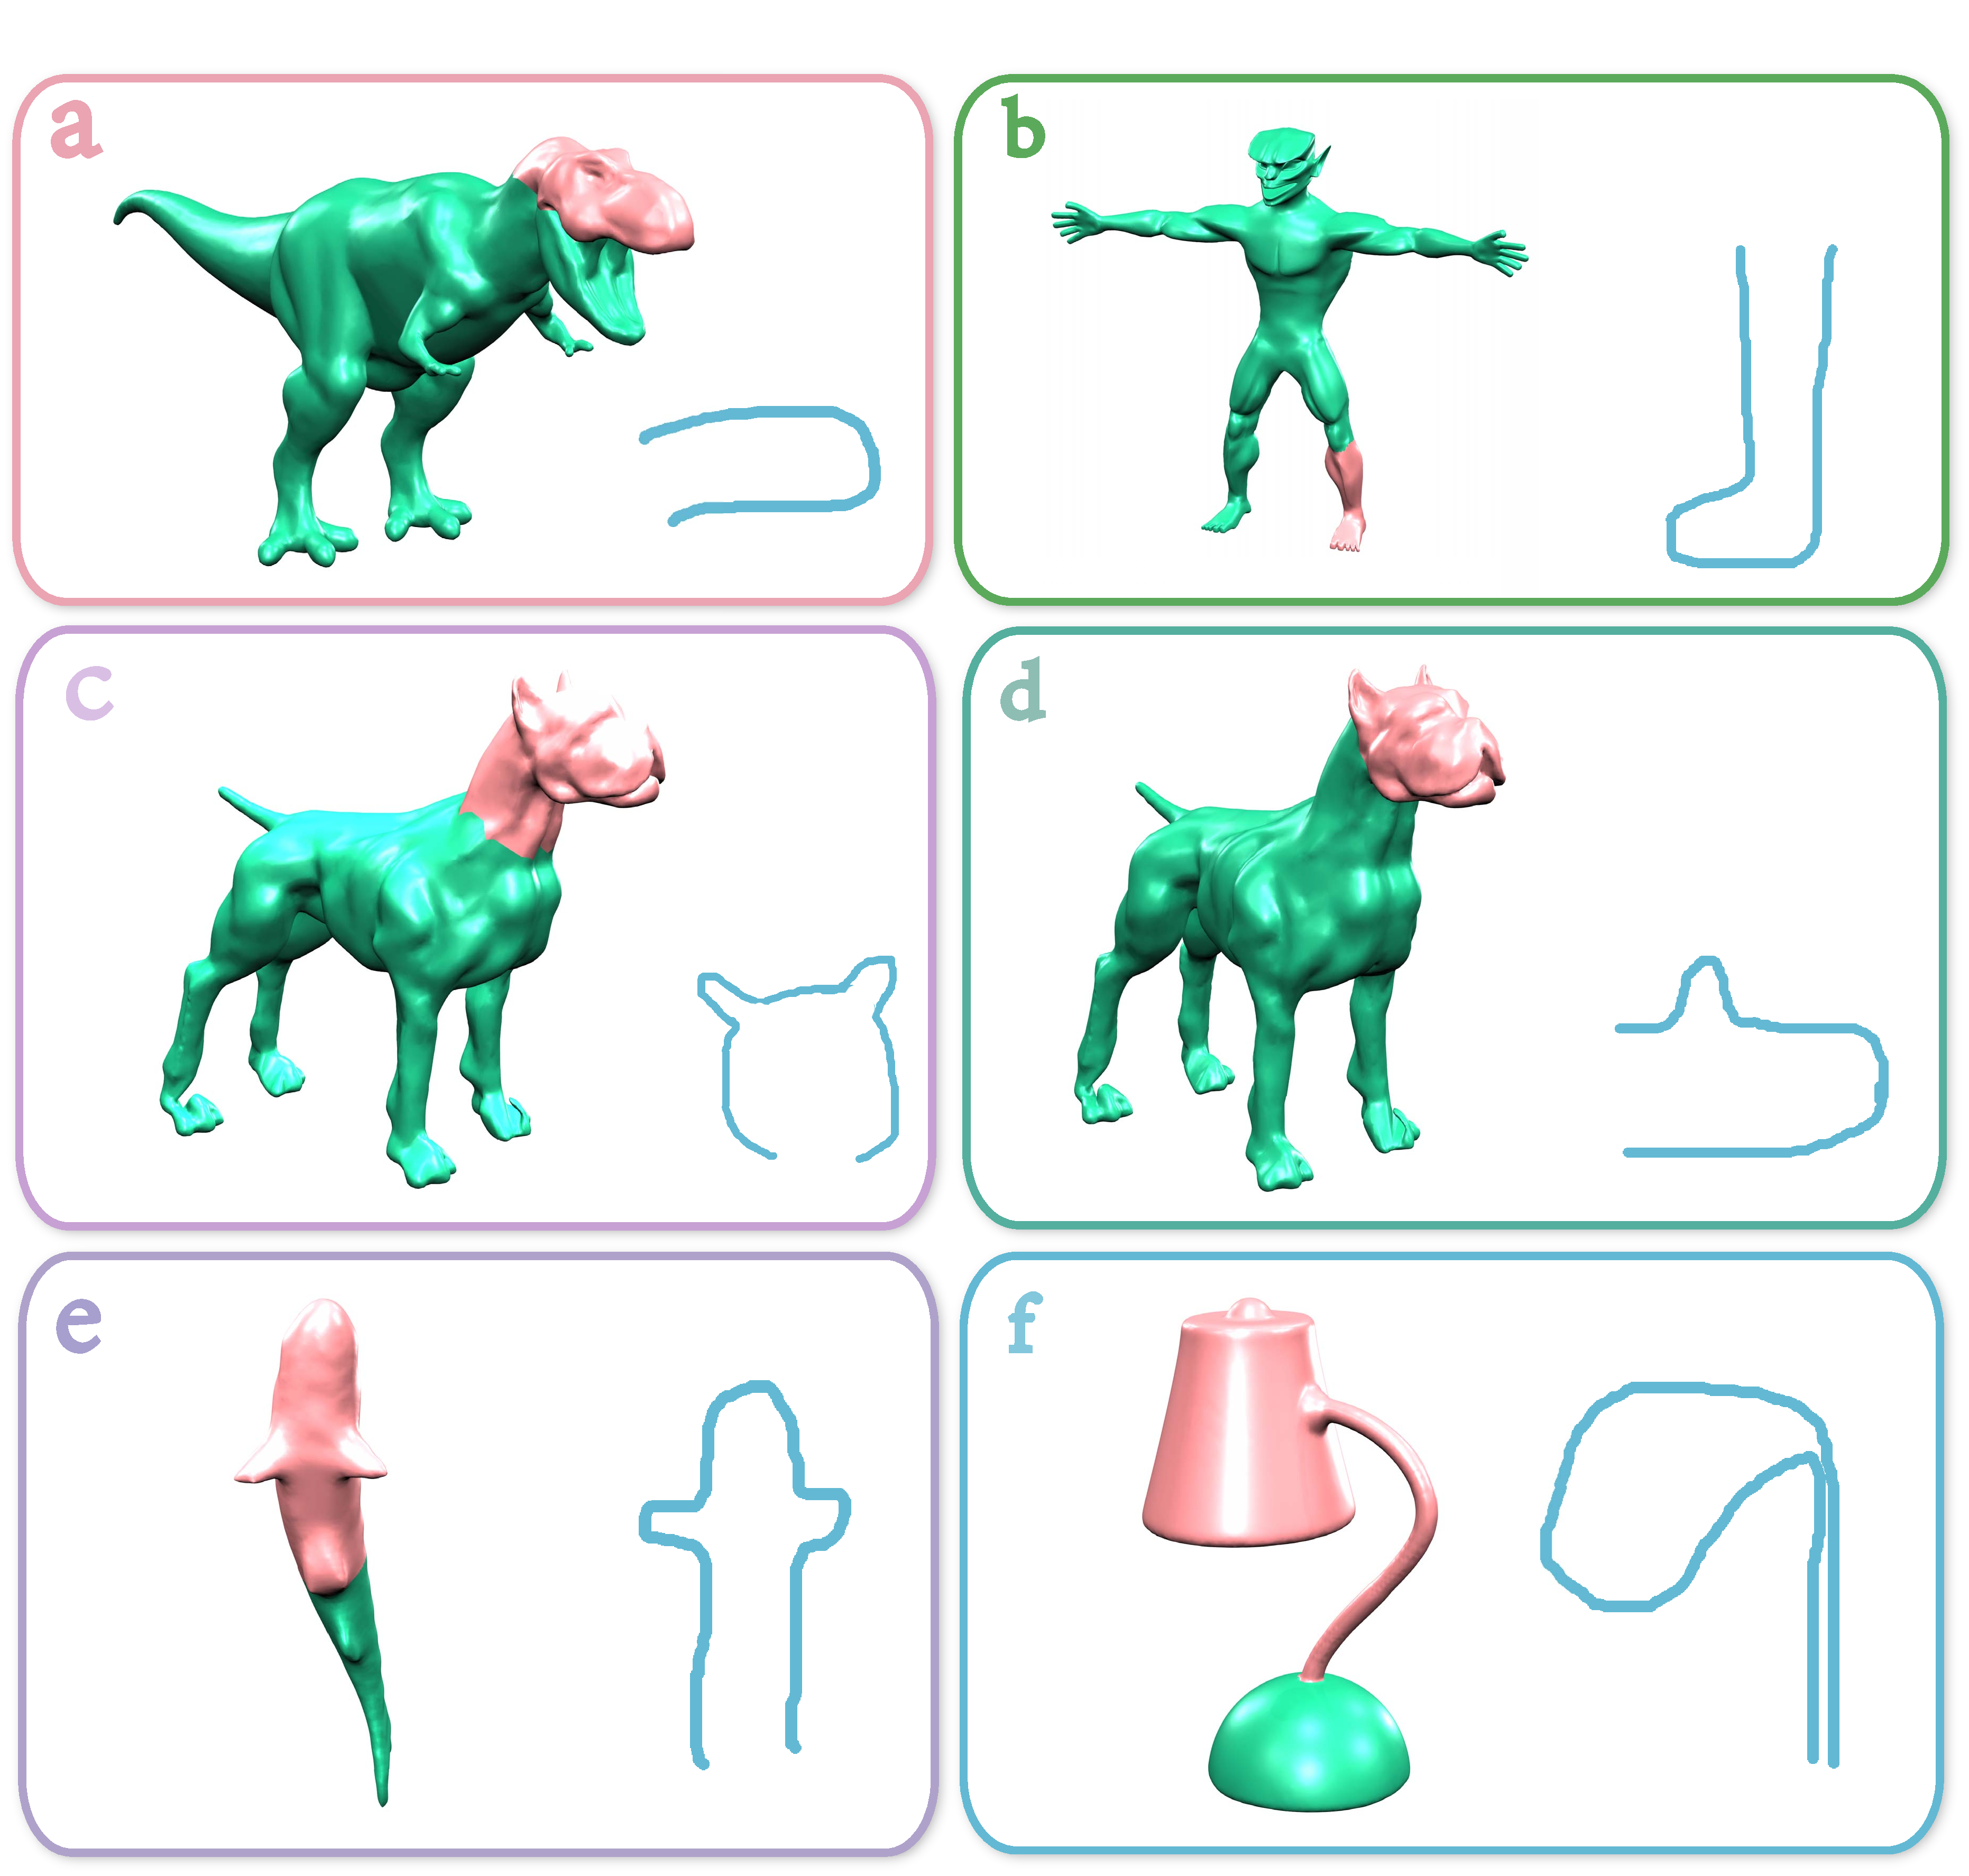
\includegraphics[width=\linewidth]{./Material/IrreWay.pdf}
\caption{Different types of parts (red) retrieved by a sketch (blue) using our algorithm. While some parts may be predefined with an automatic segmentation algorithm (d), others are irregular, defined only by the sketch (a,e), and yet others combine multiple ``standard'' segments (b: shin + foot, c: head + neck, f: shade + neck).}\label{fig:partseg}
\end{figure}

We address these challenges with a new \emph{super-face graph representation} (SFG) for a 3D shape. The super-face graph is a discretized yet fine-grained version of the original model. The vertices of the graph are a set of super-faces, obtained by an oversegmentation of the model that respects strong feature boundaries. While we could also work with the raw faces of the model, their combinatorial search space can be infeasibly large. Hence, we find candidate parts as combinations of super-faces, and subsequently refine the part boundaries down to the level of individual faces (Section \ref{sec:partrefinement}).

Edges of the graph connect pairs of adjacent super-faces. The weight of an edge indicates how frequently the super-face pair co-occurs in a single segment produced by a randomized segmentation algorithm (Figure \ref{fig:SFG}).

\begin{figure}[b]\centering
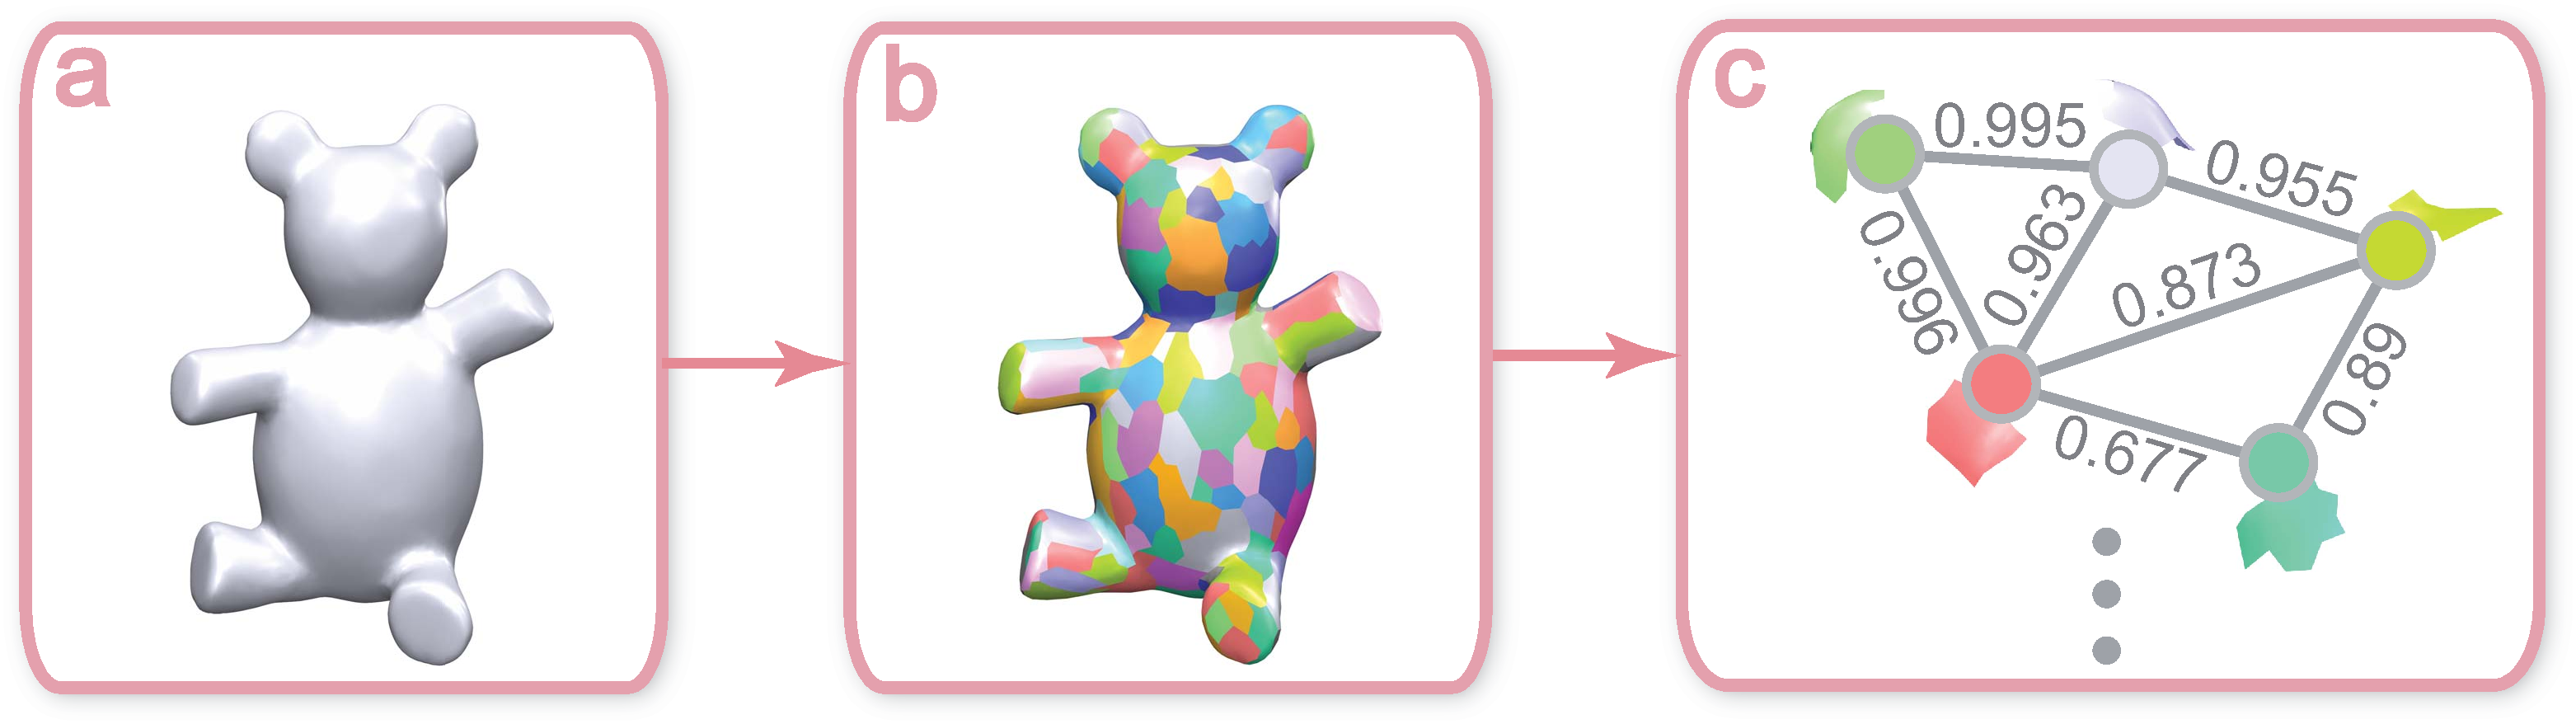
\includegraphics[width=\linewidth]{./Material/SFG.pdf}
\caption{The construction of the super-face graph for a 3D shape. Given the Teddy model (a), we partition it into a large number of super-faces (b). Each super-face is a node of the graph. Adjacent super-faces are connected by a weighted graph edge (c).}\label{fig:SFG}
\end{figure}

The super-face graph gives us a probabilistic prior for merging adjacent superfaces into larger patches to represent an arbitrary but not implausible or disconnected part of the shape. We generate the super-face graph representations of all database models in the offline phase.

%%%%%%%%%%%%%%%%%%%%%%%%%%%%%%%%%%%%%%%%%%%%%%%%%%%%%%
\subsection{Super-Face Graph Representation}\label{subsec:sfg}

To construct the super-face graph for a shape mesh, we oversegment the mesh into $N$ patches~\cite{jointshapesegmentationhuangqixingsg2011} (we experimented with $N = 50$, $100$ and $200$) and take each patch as a super-face (a vertex of the graph). Each pair of adjacent super-faces is connected by a graph edge.

\begin{figure}[b]\centering
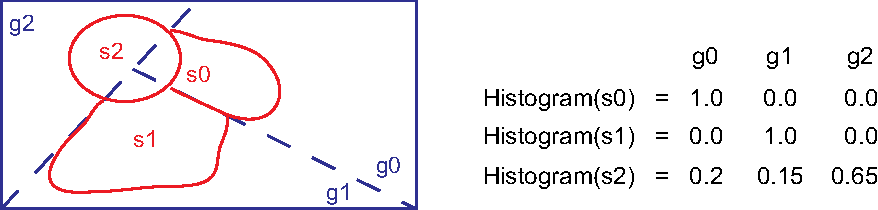
\includegraphics[width=1.0\linewidth]{./Material/Consistency.pdf}
\caption{Distributions of super-faces on segments. $s_0$, $s_1$, and $s_2$ are the super-faces. $g_0$, $g_1$, and $g_2$ are the segments generated by the randomized segmentation on the shape.}\label{fig:Consistency}
\end{figure}

To compute edge weights between nodes, we generate $900$ randomized segmentations~\cite{randomizedcutsfunkhousertog2008} over the shape with the number of segments varying from $2$ to $10$. Given a segmentation, we construct a histogram for each super-face, describing its segment memberships. Each bin of the histogram corresponds to a segment, and the value of the bin is the fractional area of the super-face lying within the segment (Figure \ref{fig:Consistency}). Mathematically, the bin value $h_s^g$ of a super-face $s$, for a segment $g$, is defined as:
\[h_s^g = \frac{{\sum\limits_{f ~\in~ Faces(g) \cap Faces(s)} {Area\left( {f} \right)} }}{{\sum\limits_{f ~\in~ Faces(s)} {Area\left( {f} \right)} }},\]
%\[h_s^g = \frac{{\sum\limits_{f \in Faces\left( g \right) \cap Faces\left( s \right)} {Area\left( f \right)} }}{{\sum\limits_{f \in Faces\left( s \right)} {Area\left( f \right)} }},\]
where $Faces(x)$ is the set of mesh faces in $x$, and $Area(f)$ is the area of face $f$.

These histograms serve as feature vectors for determining the probability that two super-faces may lie in the same segment. We define $P(s,s')$ as the probability that two adjacent super-faces $s$ and $s'$ lie in the same segment, and it is defined via the ${\chi ^2}$ distance between their histograms $H$ and $H'$:
\[{P}\left( {s,s'} \right) = 1 - {\chi ^2}\left( {H,H'} \right) = 1 - \frac{1}{2}\sum\limits_{{g_i} \in G} {\frac{{{{\left( {h_s^{{g_i}} - h_{s'}^{{g_i}}} \right)}^2}}}{{{{\left( {h_s^{{g_i}} + h_{s'}^{{g_i}}} \right)}^2}}}}, \]
where $G = \left\{ {{g_i}\left| {1 \le i \le N} \right.} \right\}$ is the set of segments generated by the randomized segmentation, $g_i$ is the $i$th segment, and $N$ is the number of segments.

To calculate the edge weight between two adjacent super-faces, we first accumulate the consistency scores over all the different randomized segmentations, and then normalize it using the number of randomized segmentation operations.

%--------------------------
\subsection{Fuzzy Part Identification}
As a first step, we use the SFG to extract a rough approximation of the part corresponding to a matched contour section. We can convert an open section to a closed one by drawing a line between its ends. This forms a natural perceptual boundary for the projection of the desired part.

Now, we start with any super-face adjacent to the center of the contour and perform a flood fill, gathering all super-faces whose projections lie within the closed contour obtained above.

We must handle several complications here. First, the contour section may be depth-discontinuous, spanning multiple isolated parts in 3D (Figure \ref{fig:ComplexCtour}(a)). Second, the contour section may enclose empty space that is not accounted for in the sketch (the blue and green sections in Figure \ref{fig:ComplexCtour}(b)). Third, the same sketch may match multiple instances of the same part (Figure \ref{fig:ComplexCtour}(c)). To address these issues, we filter out invalid parts and collapse multiple instances into a single part. \hl{The invalid parts generated with depth-discontinuous contour sections are identified by a group of isolated super-faces. This kind of parts are discarded. The multiple instances of the same part (Figure }\ref{fig:ComplexCtour}\hl{(c)) are identified by matching the sets of the super-faces. The repetitive instances are removed.}

\begin{figure}\centering
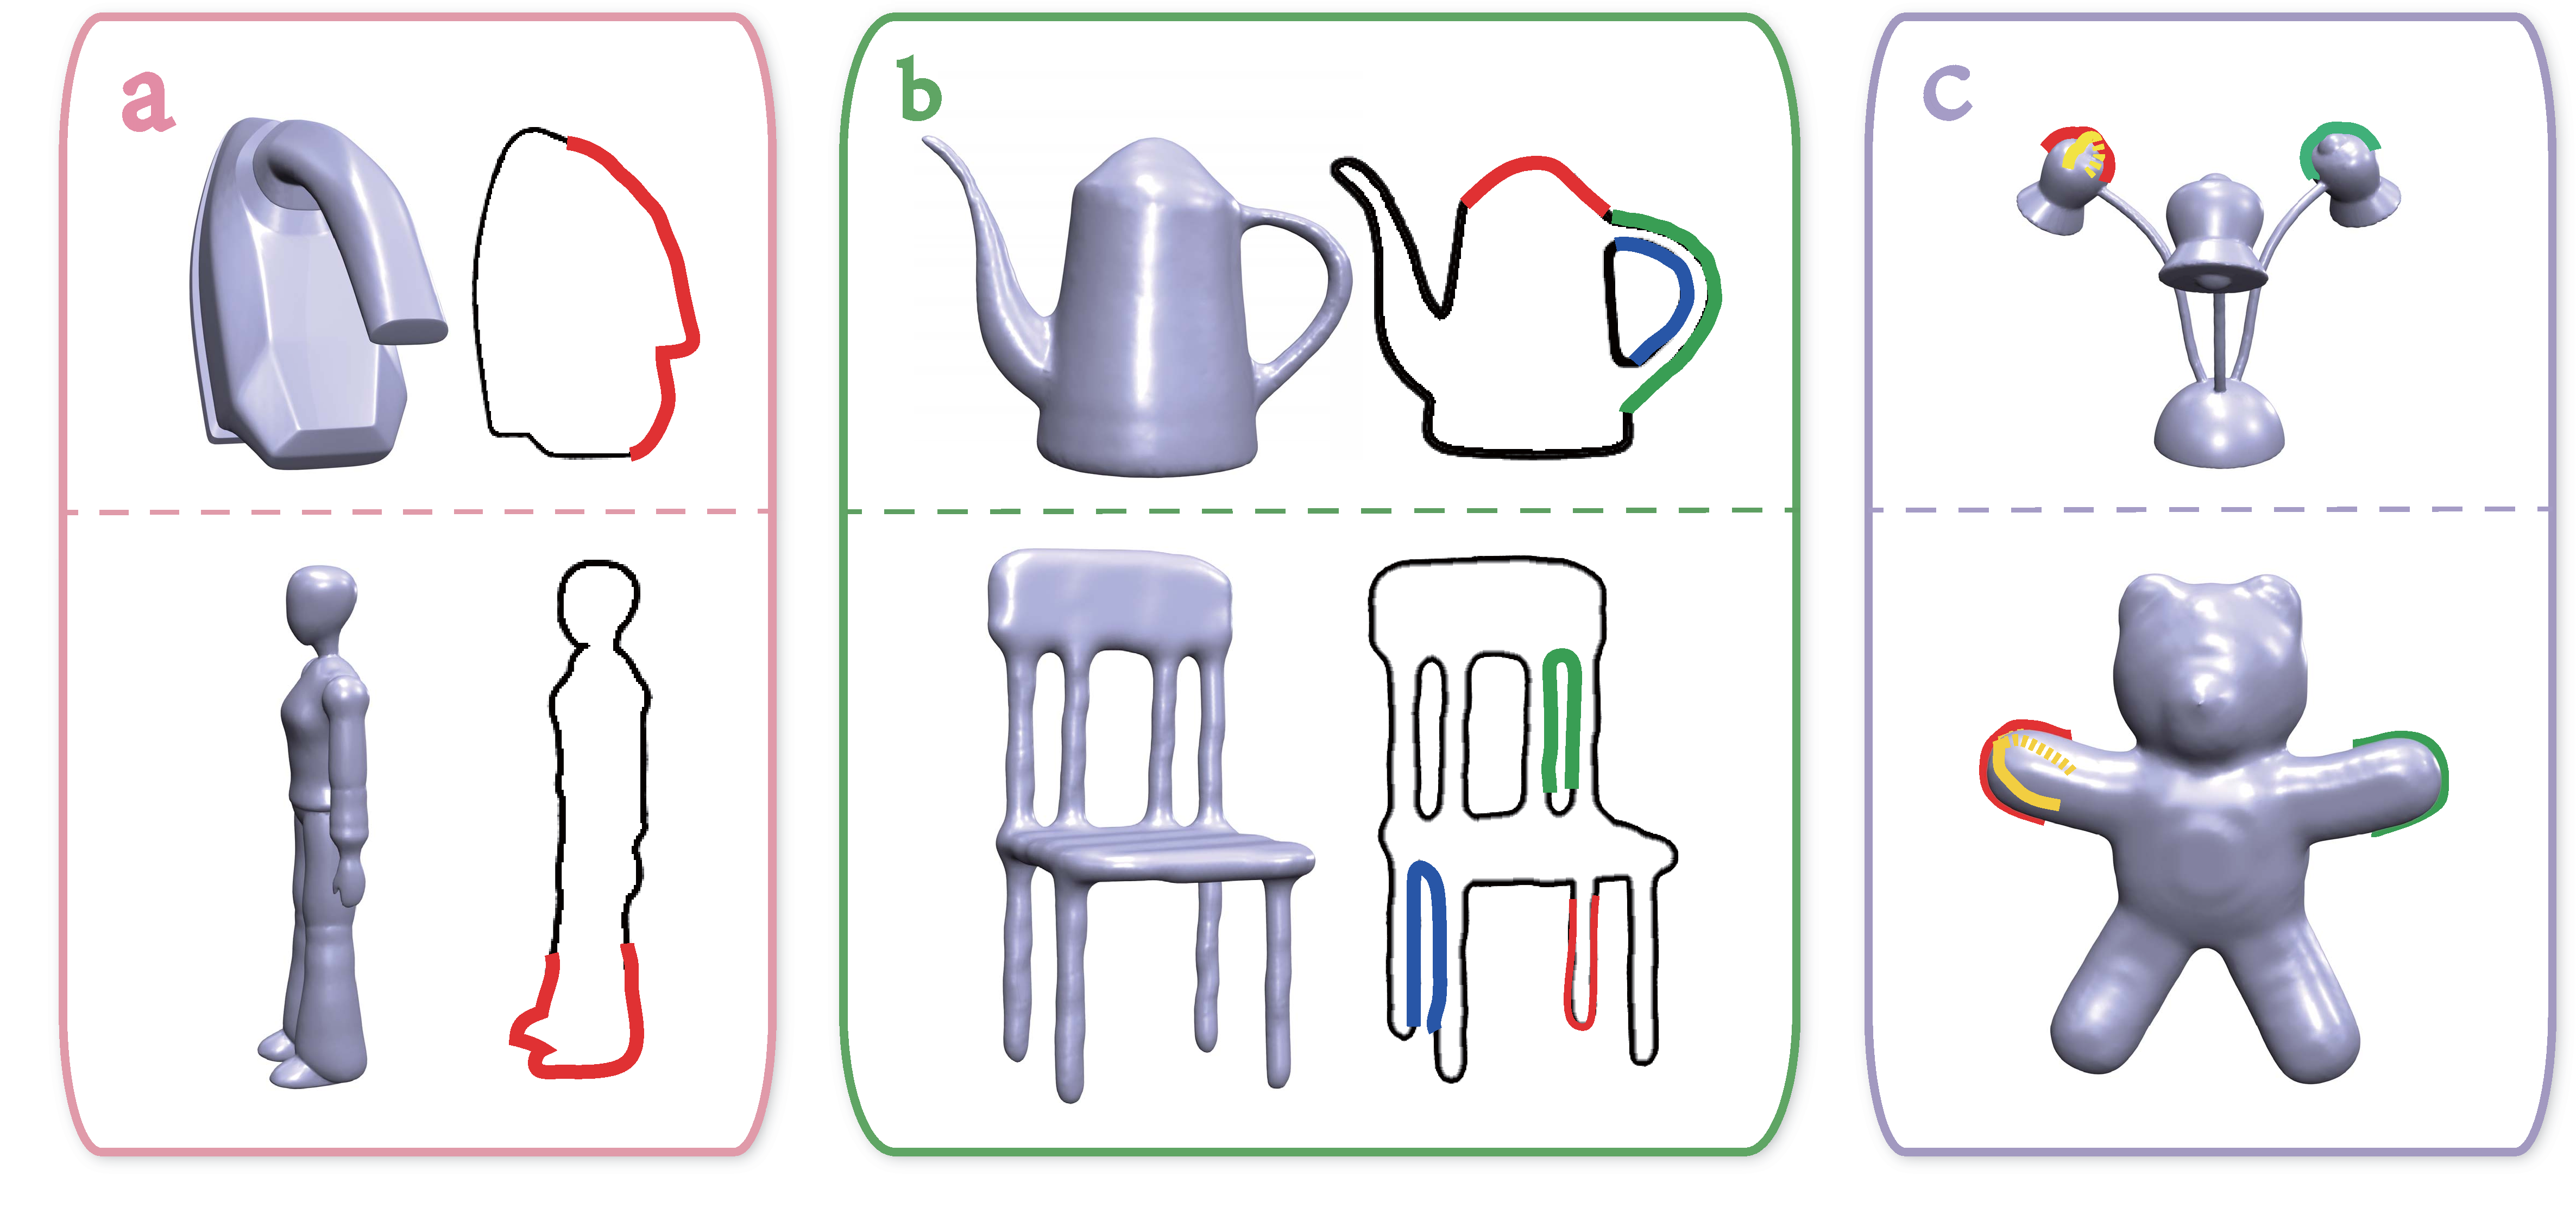
\includegraphics[width=\linewidth]{./Material/ComplexCtour.pdf}
\caption{Illustrations of the complexity of contours and their relationship. Depth-discontinuous contour sections are shown in (a). Topologically different contour sections are illustrated in (b). Isolated contour sections are shown in (c).}\label{fig:ComplexCtour}
\end{figure}

\subsection{Coarse-to-Fine Boundary Refinement}
\label{sec:partrefinement}
Once an approximate part is identified, we segment it from the model and refine its boundary to better match the sketch and respect local geometric cues. We take the following constraints into consideration:
\begin{itemize}
  \item \textbf{Contour closure.} As noted above, the line joining the ends of a contour section forms a natural perceptual boundary for the part. Hence, the part's projection should respect this line as much as possible.
  \item \textbf{Super-face co-occurrence.} If two super-faces regularly co-occur in the same segment of a random segmentation, they should probably both be retained or both excluded from the part. This acts as a shape prior.
  \item \textbf{Concavity.} Shape concavity information plays an important role in achieving high-quality segmentation as concave creases and seams are generally regarded as natural segmentation boundaries by humans \cite{concavityawareyouyitvcg2012}.
  \item \textbf{Smoothness.} The boundary should avoid sharp zigzags.
\end{itemize}

We propose a novel coarse-to-fine strategy that optimizes the fuzzy part boundary in two steps: (1) optimize the set of boundary superfaces according to perceptual and co-occurrence priors; and (2) further refine the boundary at the level of individual faces, using the remaining constraints.

\subsubsection{Coarse Level Extraction}
We formulate the coarse level part extraction as a binary labeling problem which can be solved by minimizing a Gibbs energy $E_{c}$:
\[E_{c} = \sum\limits_{{i} \in V} {{E_{1}}\left( {{l_{i}}} \right)}  + \sum\limits_{\left( {i,j} \right) \in E} {{E_{2}}\left( {{l_{i}},{l_{j}}} \right)} ,\]
where $V$ and $E$ represent the nodes and edges of the super face graph $\mathcal{G}$, respectively, $E_{1}(l_{i})$ is the likelihood energy encoding the cost when the label of node $i$ is $l_{i}$, and ${E_{2}}\left( {{l_{i}},{l_{j}}} \right)$ is the prior energy denoting the cost when the labels of adjacent nodes $i$ and $j$ are $l_{i}$ and $l_{j}$, respectively. $E_1$ is defined as follows:
\[{E_1}\left( {{l_i}} \right) = \left\{ {\begin{array}{*{20}{c}}
   { - \ln {\mathcal{P}}\left( i \right),} & {{l_i} = 1,}  \\
   { - \ln \left( {1 - {\mathcal{P}}\left( i \right)} \right),} & {{l_i} = 0,}  \\
\end{array}} \right.\]
where $\mathcal{P} \left( i \right)$ is the probability of assigning label $1$ to node $i$. According to the {\em contour closure} constraint, $\mathcal{P}(i)$ is defined as the fractional area of the $i$th super-face lying within the contour closure:
\[{\mathcal{P}}\left( i \right) = \frac{{Area_{proj}^{in}\left( i \right)}}{{Are{a_{proj}}\left( i \right)}},\]
where $Area_{proj}^{in} \left( i \right)$ is the area of the projection of the $i$th super-face overlapping with the contour closure, $Area_{proj} \left( i \right)$ is the area of the projection of the $i$th super-face. $E_2$ is defined according to the {\em super-face co-occurrence} constraint:
\[{E_2}\left( {{l_i},{l_j}} \right) = \left\{ {\begin{array}{*{20}{c}}
   {0,} & {{l_i} = {l_j},}  \\
   {{e_{ij}},} & {{l_i} \ne {l_j},}  \\
\end{array}} \right.\]
where $e_{ij}$ is the edge weight of the SFG. We solve $E_{c}$ using binary graph cut \cite{anexperimentalcomparisonboykovpami2004}.
%--------------------------
\subsubsection{Fine Level Extraction}
\label{sec:finelevelextraction}
After obtaining the coarse level part, we map each boundary super face of $\mathcal{G}$ onto a vertex in the original surface that is closest to the center of the super face. For an edge $e$ in $\mathcal{G}$, let $v_{1}$ and $v_{2}$ be the projections of its nodes on the original surface. We propagate from $v_{1}$ toward $v_{2}$ by iteratively finding the neighbour whose projection on the line $v_{1}v_{2}$ is closest to $v_{2}$.

We then refine the obtained boundary in an iterative manner to minimize the following energy:
$$
E_{f}=E_{v}+E_{s},
$$
where $E_{v}$ is the concavity energy, and $E_{s}$ is the smoothness energy. $E_{v}$ is defined as the sum of all boundary edge's concavity energy \cite{hierarchicalmeshdecompositionayellettog2003}:
$$
E_{v}=\sum_{e\in \partial Q}\eta(1+\cos\alpha_{e})|e|,
$$
where $e$ represents an edge on the boundary of the candidate part $Q$, $\left| \cdot \right|$ represents the length of $e$, $\alpha_{e}$ is the dihedral angle of $e$, $\eta=0.1$ when $e$ is concave, otherwise $\eta=1.0$.
$E_{s}$ is defined as:
\[{E_s} = \sum\limits_{v \in \partial Q} {\left| {\sin\left\langle {{e_l},{e_r}} \right\rangle } \right|},\]
where $v$ is a vertex on the boundary $Q$, $e_l$ is an edge on $Q$ pointing to $v$, and $e_r$ is \st{an other} \hl{another} edge on $Q$ starting from $v$. We apply snake operations on the boundary vertices to minimize the energy $E_{f}$ \cite{CGF:CGF947}.
